\chapter{Speaker Verification Systems}
\label{ch:speaker-verification-system}

%TODO remodelar, retirando tudo sobre Speaker IDENTIFICATION

The process of speaker recognition lies on the field of pattern classification, with the speaker's utterance (a speech signal) as input for a classifier. This decision may be, given a speech signal $\dvec{Y}$ produced by a speaker $\mathcal{S}$ and a set $\dvec{\mathcal{S}} = \{\mathcal{S}_1, ..., \mathcal{S}_S\}$ of enrolled users, ``identify $\mathcal{S}$ as $\mathcal{S}_i$ if $i = \arg\max_j P(\mathcal{S}_j|\dvec{Y})$". This is a case of speaker identification and the output is a $\mathcal{S}_i$ from $\dvec{\mathcal{S}}$. Another type of decision is ``accept $\mathcal{S}$ as $\mathcal{S}_i$ if $P(\mathcal{S}_i|\dvec{Y}) \geq \alpha$", where $\mathcal{S}_i$ is the claimed identity of $\mathcal{S}$. This is a speaker verification decision. Both are covered in this chapter.

\section{Basic Concepts}

Before explain the architecture of both types of recognizers, the elucidation of some basic concepts is necessary.

\subsection{Utterance}

An utterance is a piece of speech produced by a speaker. It may be a word, a statement or any vocal sound. The terms \emph{utterance} and \emph{speech signal} sometimes are used interchangeably, but from herenow speech signal will be defined as an utterance recorded, digitalized and ready to be processed. An example is shown in \figureref{speech_signal}.

\begin{figure}[ht]
    \centering
    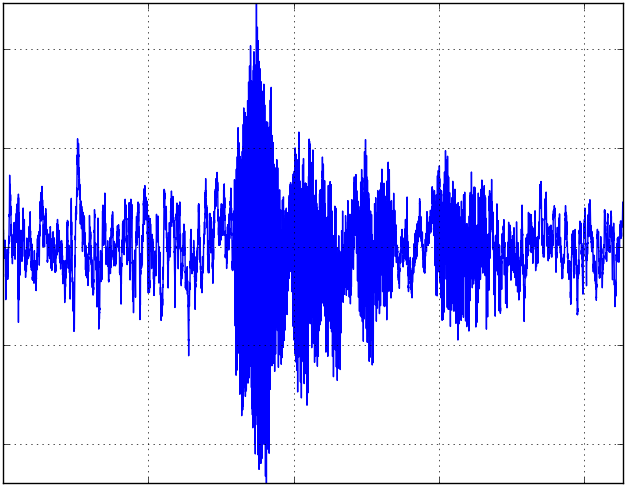
\includegraphics[width=\textwidth]{speech_signal}
    \caption{Speech signal for utterance ``karen livescu", \refbib{Woo, Park \& Hazen}{woo.park.hazen.2006}.}
    \label{fig:speech_signal}
\end{figure}

\subsection{Features}

The raw speech signal is unfit for usage by an ASR. For a correct processing, the unique features from the speaker's vocal tract are extracted, what reduces the number of variables the system needs to deal with (leading to a simpler implementation) and performs a better evaluation (prevents the curse of dimensionality). Due to the stationary properties of the speech signal when analyzed in a short period of time, it is divided in overlapping frames of small and predefined length, to avoid ``loss of significancy" in the features, \refbib{Davis \& Mermelstein}{davis.mermelstein.1980}, \refbib{Rabiner \& Schafer}{rabiner.schafer.2007}. This extraction is executed by the MFCC algorithm, explained in details in \chapterref{feature-extraction}.

\section{Speaker Identification}
\label{sec:speaker-identification}

In speaker identification, the objective of the system is to assign an identity from a set of enrolled speakers to the so far unknown speaker, using a speech signal produced by him or her. This system contains a set $\dvec{\mathcal{S}}$ and is fed with features $\dvec{X} = \{\dvec{x}_1, ..., \dvec{x}_T\}$ extracted from the speech $\dvec{Y}$ produced by the speaker $\mathcal{S}$, the one to be identified.

\begin{figure}[ht]
    \centering
    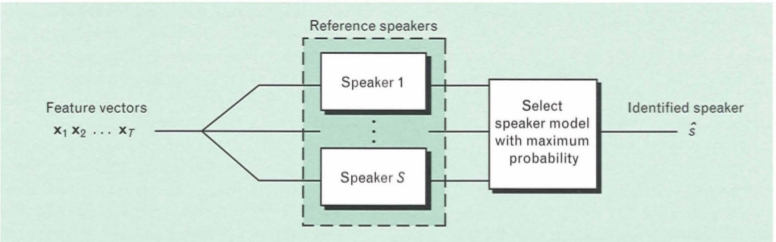
\includegraphics[width=\textwidth]{speaker-identification}
    \caption{Speaker-recognition system for identification, \refbib{Reynolds}{reynolds.1995a}.}
    \label{fig:speaker-identification}
\end{figure}

\noindent The system is the closed set speaker identification described in \sectionref{speaker-recognition}, and it classifies any speaker, be it an enrolled one or not. Unenrolled speakers are incorrectly identified as the speaker which model returns the highest probability. The equation to determine the identity of $\mathcal{S}$ is

\begin{equation}
    \mathcal{S}_i \text{ if } i = \arg\max_j \postprob{\mathcal{S}_j}{\dvec{X}},
    \label{eq:decision_speaker_identification}
\end{equation}

\noindent and as all speakers have the same prior probability, \equationref{decision_speaker_identification} is reduced to

\begin{equation}
    \mathcal{S}_i \text{ if } i = \arg\max_j \postpdf{\dvec{X}}{\mathcal{S}_j}.
    \label{eq:decision_speaker_identification_2}
\end{equation}

\subsection{Training}

The use of $\mathcal{S}_j$ to represent the speaker is inaccurate, because it maintains the problem in a high level of abstraction. To present a more concrete solution, it is necessary to use a model $\lambda_j$ for each $\mathcal{S}_j$. Each $\lambda_j$ is trained independently until a stop condition is fulfilled.

\subsection{Test}

Once all $\lambda_j$'s are trained, the system if able to be used for classification. \equationref{decision_speaker_identification_2} is then redefined as

\begin{equation}
    \mathcal{S}_i \text{ if } i = \arg\max_j \postpdf{\dvec{X}}{\lambda_j},
    \label{eq:decision_speaker_identification_3}
\end{equation}

\noindent and the unknown speaker receives the identity of the enrolled speaker for which $\dvec{X}$ maximizes the \textbf{likelihood} of $\lambda_j$ (see \figureref{speaker-identification}).

\section{Speaker Verification}
\label{sec:speaker-verification}

In speaker verification, $\mathcal{S}$ claims to be a particular $\mathcal{S}_i$ from $\dvec{\mathcal{S}}$. The strength of this claim resides on how similar the features $\dvec{X}$ are to the features from $\mathcal{S}_i$ ``memorized" by the system. Then a simple equation

\begin{equation}
    \postpdf{\boldsymbol{Y}}{\mathcal{S}_i} \verifytestB{\alpha}{\mathcal{S}}
    \label{eq:decision_speaker_verification}
\end{equation}

\noindent should be enough (again considering all speakers equally probable). However a subset of enrolled speakers may have vocal similarities, leading to a misclassification of one enrolled speaker as another (a false positive). To reduce the error rate, the system must decide not only if a speech signal came from the claimed speaker, but also if it came from a set composed of all other enrolled speakers.

\subsection{Likelihood Ratio Test}

Given the vector of features $\dvec{X}$, and assuming it was produced by only one speaker, the detection task can be restated as a basic test between two hypoteses, \refbib{Reynolds}{reynolds.1995b}:

\begin{description}\itemsep0pt
    \item $H_0$: $\dvec{X}$ is from the claimed speaker $\mathcal{S}_i$;
    \item $H_1$: $\dvec{X}$ is \underline{not} from the claimed speaker $\mathcal{S}_i$.
\end{description}

\noindent The optimum test to decide which hypotesis is valid is the \textbf{likelihood ratio test} between both likelihoods $\postpdf{\dvec{X}}{H_0}$ and $\postpdf{\dvec{X}}{H_1}$

\begin{equation}
    \frac{\postpdf{\dvec{X}}{H_0}}{\postpdf{\dvec{X}}{H_1}} \verifytestB{\theta}{H_0}
    \label{eq:likelihood-ratio-test}
\end{equation}

\noindent where the decision threshold for accepting or rejecting $H_0$ is $\theta$. Applying the logarithm, the behavior of the likelihood ratio is maintained and \equationref{likelihood-ratio-test} is replaced by the log-likelihood ratio

\begin{equation}
    \Lambda(\dvec{X}) = \log \postpdf{\dvec{X}}{H_0} - \log \postpdf{\dvec{X}}{H_1}.
    \label{eq:log-likelihood-ratio-test}
\end{equation}

\subsection{Training}

Once the features are extracted from the speech signal, they are used to train the models $\lambda_{hyp}$ and $\lambda_{\overline{hyp}}$ for $H_0$ and $H_1$, respectively. A high-level demonstration of the training of $\lambda_{hyp}$ (mathematical representation of $\mathcal{S}_i$) is shown in \figureref{speaker-verification-training}.

\begin{figure}[ht]
    \centering
    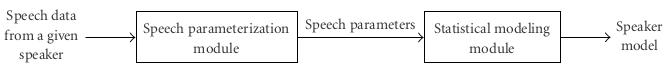
\includegraphics[width=\textwidth]{speaker-verification-training}
    \caption{The statistical model of $\mathcal{S}$ is created from the speech signal $\dvec{Y}$, \refbib{Bimbot et. al.}{bimbot.et.al.2004}.}
    \label{fig:speaker-verification-training}
\end{figure}

Due to $\lambda_{hyp}$ be a model of $\mathcal{S}_i$, the features used for training (i.e., estimate $p(\dvec{X}|\lambda_{hyp})$) are extracted from speech signals produced by $\mathcal{S}_i$. The model $\lambda_{\overline{hyp}}$, however, is not well-defined. It should be composed of the features extracted from speech signals from all other speakers except $\mathcal{S}_i$, but creating a single $\lambda_{\overline{hyp}}$ for each speaker is complicated and with no expressive gain. Instead, what is normally done is use all speakers to generate a background model $\lambda_{bkg}$, \refbib{Reynolds}{reynolds.1997}, in which the weight of each $\mathcal{S}_i$ is minimized.

\subsection{Test}

As seen in \equationref{likelihood-ratio-test}, the decision process is based on a function \emph{Score}. Replacing each $H_j$ for its corresponding model, the likelihood of a $\lambda_j$ given $\dvec{X}$ can be written as

\begin{equation}
    p(\dvec{X}|\lambda_j) = \prod_{t=1}^T p(\dvec{x}_t|\lambda_j).
    \label{eq:likelihood-prod}
\end{equation}

\noindent Using the logarithm function, \equationref{likelihood-prod} becomes

\begin{equation}
    \log p(\dvec{X}|\lambda_j) = \frac{1}{T} \sum_{t=1}^T \log p(\dvec{x}_t|\lambda_j),
    \label{eq:log-likelihood-sum}
\end{equation}

\noindent where the term $\frac{1}{T}$ is used to normalize the log-likelihood to the duration of the speech signal. That said, the likelihood ratio given by \equationref{log-likelihood-ratio-test} becomes

\begin{equation}
    \Lambda(\dvec{X}) = \log p(\dvec{X}|\lambda_{hyp}) - \log p(\dvec{X}|\lambda_{bkg}),
    \label{eq:score_of_X}
\end{equation}

\noindent and the speaker is accepted if $\Lambda(\dvec{X}) \geq \log \theta$, for an arbitrary value of $\theta$.